\chapter{Pruebas de concepto}
\section{Propuestas}
Una vez se han testeado y analizado las diferentes tecnologías surgen diferentes ideas como prueba de concepto en función de las características particulares de cada tecnología. Las cuales son enumeradas a continuación:

\begin{itemize}
\item Desarrollo de un \textit{plugin} capaz de gestionar los \textit{cloud anchor} en interiores y almacenar la información durante un período de tiempo ajustable a las necesidades del producto. Será capaz de identificar estas posiciones \textit{online} y \textit{offline} mediante una base de datos almacenada tanto en servidor como en local si fuese necesario. Plataformas deseables: Android (prioritario) y iOS. 
\item API de alto nivel que permite desarrollar de manera más versátil y sencilla aplicaciones en realidad aumentada teniendo compatibilidad plena entre ARKit y ARCore. El usuario será capaz de desarrollar una aplicación en realidad aumentada completa sin apenas líneas de código ya sea mediante \textit{blueprints} o módulos.
\item Juego multijugador con \textit{Cloud Anchors}. Juego en el que dos jugadores o más compiten por conseguir más puntos por destruir edificios. (Inspirado en Bombardero - Amstrad CPC)
\item Plataforma de realidad aumentada: permitirá al usuario acceder en el momento a diferentes contenidos ya sean vídeos, juegos o experiencias sin necesidad de salir de la aplicación. Esta idea estaba pensada para el uso con unas gafas de AR y mando inalámbrico para el control del dispositivo. Inspirado en Google DayDream.
\item Reconocimiento de objetos.
\item Proceso de montaje de muebles paso a paso del en realidad aumentada.
\end{itemize}

\clearpage
\section{Primeros prototipos}
En esta sección hablaremos de los prototipos que se han desarrollado previamente a las tres aplicaciones cerradas.\\

Con el fin de iniciarnos en el desarrollo de aplicaciones de realidad aumentada, decidimos que la mejor idea sería empezar por implementar a modo de prueba algunos prototipos de programas que utilizasen la realidad aumentada con marcadores. Lo hicimos así para ir avanzando por las diferentes etapas por las que ha pasado este campo en todo su proceso evolutivo.

\subsection{Harry Potter}
Después de descartar ARToolkit por no encontrar documentación actualizada del mismo y estar bastante obsoleto con respecto a otras librerías, nos decantamos por hacer las pruebas con Vuforia, que tiene soporte tanto para realidad aumentada con marcadores como sin ellos. Además, la documentación es reciente y ofrece una serie de posibilidades que nos interesaba aprovechar, como por ejemplo su integración con Unity3D.\\

Para implementar los prototipos pensamos en aplicaciones que fueran rápidas de codificar, pero que pudieran aportar algo interesante a los ojos de los usuarios. Tras un tiempo de debate encontramos curiosa la idea de que “escaneando” con el móvil un cartel o las viñetas de un cómic se pudiese obtener información no presente a simple vista en el mundo real, aportándole una capa más de profundidad y dinamismo a la experiencia del observador. A continuación comentamos el proceso de desarrollo.\\

Suscribiéndonos a la web de Vuforia se nos da la posibilidad de crear una base de datos con imágenes que nosotros mismos tomemos o escojamos para la aplicación. Este servicio de Vuforia ofrece un número limitado de bases de datos que podemos crear, pero es posible expandirlo y encontrar otras funcionalidades con los planes Basic o Pro. En nuestro caso no lo consideramos necesario y procedimos a buscar una imagen que nos sirviese como marcador. En esta primera aproximación nos basamos en los periódicos mágicos que aparecen en la saga de películas de Harry Potter y encontramos la página del periódico en la que aparece el prisionero de Azkaban (la cárcel de este universo literario). Al subir al servidor de Vuforia la imagen, la web te muestra una estimación de cuánto de reconocible es el marcador basándose en el contraste que existe entre la saturación de las distintas partes en las que divide la foto. De esta forma puedes decidir como desarrollador si vas a utilizar cierta imagen como marcador o vas a buscar otra con unas características mejores y que haga la experiencia más cómoda de cara al usuario.\\

Como explicábamos, nosotros utilizamos la imagen que incluimos en la figura \ref{Azkaban}, recortando el cuadrado en el que aparece la foto del preso que es la que utilizaremos como marcador. A continuación tuvimos que buscar el fragmento animado del periódico que aparece en la película, que no nos llevó mucho tiempo puesto que debido a la popularidad de la saga estaba disponible en varias páginas web. Después ajustamos con un editor de video el tamaño del gif animado para que coincidiera con las dimensiones de la foto, como podemos observar en la imagen de la derecha de la figura \ref{Azkaban}.\\

\begin{figure}[H]
    \centering
    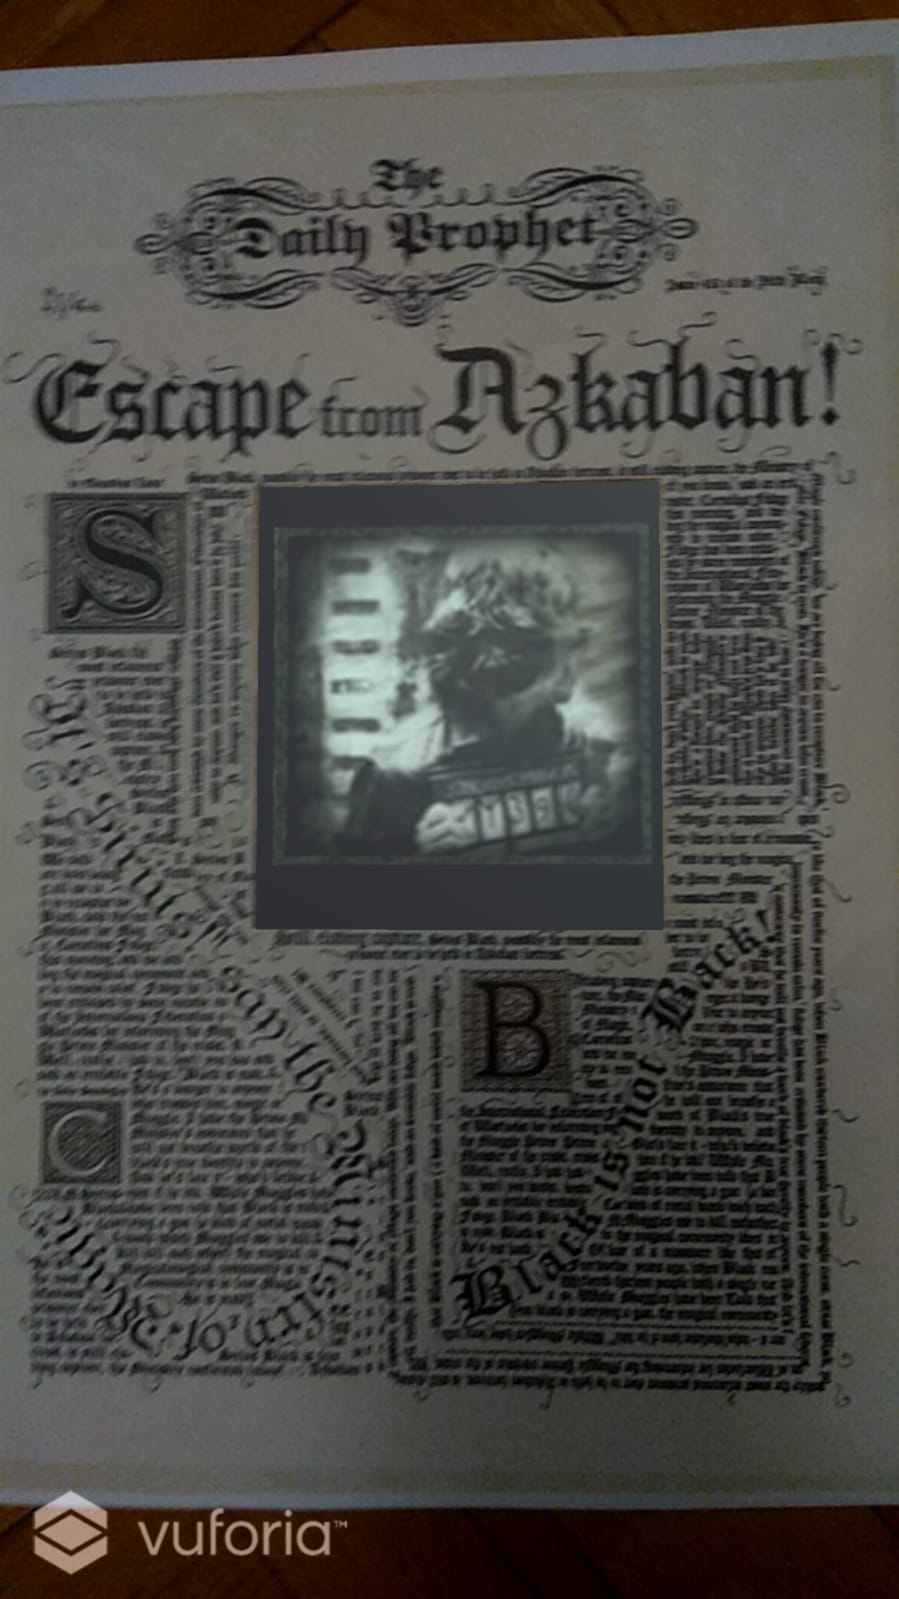
\includegraphics[width=0.4\linewidth]{Images/Azkaban.jpeg}
    \caption{Aplicación del periódico de Harry Potter}
    \label{Azkaban}
\end{figure}

Ahora viene el momento de utilizar Unity. Desde el editor, y con el paquete de Vuforia instalado procedimos a importar la base de datos que nos da Vuforia con la ilustración convertida en marcador. Realizar un uso básico y a modo de prueba de esta librería para el desarrollo de un ejemplo en realidad aumentada es bastante sencillo y animamos a cualquier persona que sienta curiosidad a seguir estos pasos, ya que solo requiere algunos conocimientos de cómo usar el editor de este motor de videojuegos.\\

Necesitamos en la escena un objeto que sea del tipo \textit{AR Camera}, que se encargará de renderizar la escena y detectar los marcadores. Usando este objeto podemos prescindir de la cámara tradicional. A continuación introdujimos el objeto \textit{Image Target}, también dentro del paquete de Vuforia y lo configuramos para que el componente \textit{Image Target Behaviour} utilice la base de datos que tenemos y la imagen que le corresponde. Como hijo del \textit{Image Target} incluimos el objeto virtual que queremos que aparezca al encontrar el marcador. En este caso, un objeto del tipo \textit{Quad} (es decir, un rectángulo vacío) nos servirá. Ajustamos el ancho y el alto al tamaño del padre y le añadimos el componente \textit{Video Player} para que reproduzca el gif animado. Con esto sólo necesitaríamos compilar la aplicación y pasar el archivo apk a un móvil que lo soporte para probar la aplicación.\\

\textbf{Se pueden ver los resultados en el video \url{https://vimeo.com/331236805}.}

\subsection{DragonBall}
La siguiente aplicación que desarrollamos está impulsada por la idea de leer un cómic en realidad aumentada. Utilizamos una página del manga de Dragon Ball para este ejemplo y le aplicamos básicamente el mismo procedimiento que al programa anterior, aunque con un par de excepciones.\\

En primer lugar, escogimos una página con unas viñetas lo suficientemente nítidas como para que los marcadores fueran de calidad. Una vez seleccionada (figura \ref{DBZ}) continuamos con el proceso de subida al servidor de Vuforia para obtener la base de datos. La parte difícil vino a continuación, pues tuvimos que encontrar el capítulo de la serie animada en el que sucedieran los hechos de esa página del cómic, para después recortar los fragmentos correspondientes a cada viñeta y ajustar el breve video de cada una al tamaño justo de la misma. Una vez teníamos todas las materias primas ya sólo había que introducirlas en el editor de Unity, creando esta vez cuatro \textit{Target Images} (uno para cada viñeta) y un \textit{Quad} con el video propio para cada uno.\\

Estamos especialmente contentos con esta demostración, ya que sin ser muy difícil de implementar, el resultado es muy vistoso y puede llegar a convertirse en una forma de ampliar la inmersión o mejorar la experiencia de los lectores habituales.
\begin{figure}[H]
    \centering
    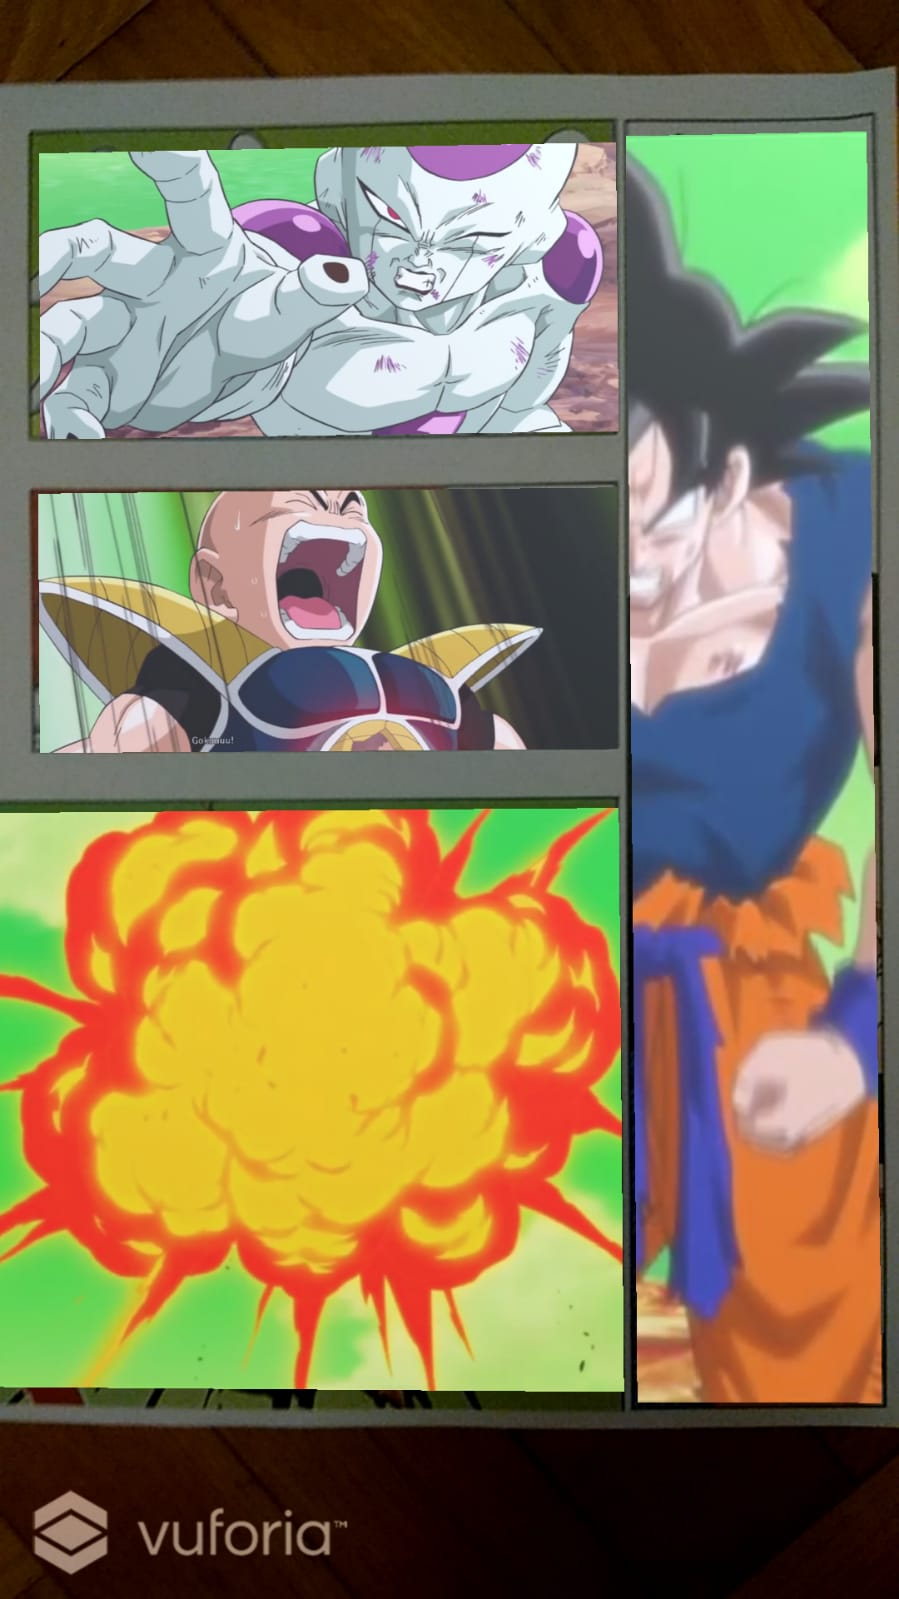
\includegraphics[width=0.3\linewidth]{Images/DragonBall.jpeg}
    \caption{Página del cómic con RA}
    \label{DBZ}
\end{figure}

Cabe destacar que actualmente la tecnología está limitada en este ámbito, ya que pese a que muchos dispositivos como tabletas o móviles soportan la realidad aumentada sin marcadores es de cierta manera incómodo tener que estar enfocando con la cámara al lugar en cuestión para obtener la información o la experiencia adicional y resulta cansado después de unos cuantos usos. Sin embargo, con dispositivos similares a las \textit{Google Glass}, que incorporen realidad aumentada y puedan llevarse siempre puestas, el mercado de este tipo de aplicaciones crecería radicalmente y se popularizaría enormemente su uso.

\textbf{Se pueden ver los resultados en el video \url{https://vimeo.com/331236593}.}

\subsection{Juego de cartas Yu-gi-oh}
Llegados a este punto, queríamos comprobar cómo sería el desarrollo de un juego que utiliza realidad aumentada con marcadores. Nos basamos para ello en el juego de cartas de Yu-Gi-Oh, que tiene su origen en un cómic japonés del mismo nombre y que alcanzó gran popularidad en la década de los 2000 en todo el mundo. El juego es de temática similar al de las cartas Magic, en el que cada carta representa un monstruo, cada uno con sus propios atributos, valores de ataque y defensa y otras características, que se enfrentan contra los monstruos del oponente siguiendo un sistema de reglas y turnos bastante complejo. Además de las cartas de monstruo existen otras que modifican los valores de las mismas o tienen otros efectos en la partida. Para facilitar el desarrollo, simplificamos todas estas condiciones y nos centramos en algunos aspectos esenciales: la partida se va sucediendo por turnos, las criaturas pertenecen a uno u otro jugador según su posición en la mesa y dentro de un turno el jugador puede decidir si el monstruo que está bajo su control ataca o defiende.\\

Lo verdaderamente interesante de este juego es que en la saga de cómic (y posterior serie animada de televisión) los jugadores juegan sobre un tablero electrónico sobre el que colocan las cartas y aparece una representación holográfica de las criaturas de las mismas. Esta tecnología de ciencia ficción se escapa un poco de nuestro alcance y presupuesto, pero sí que podemos intentar una recreación más simple con nuestros conocimientos de realidad aumentada y ver a los monstruos por medio de la pantalla de nuestros dispositivos móviles, como ya hicieron anteriormente juegos como Pokémon Go en 2016 o Invizimals en 2009.\\

Para desarrollar esta aplicación volvimos a utilizar el motor Unity con Vuforia. Utilizamos dos cartas del juego como marcadores para que durante el uso del programa proyectaran los modelos 3D de los monstruos correspondientes. Para los modelos buscamos algunas de las criaturas más conocidas de la franquicia y así evitamos tener que realizar nosotros a mano el proceso de modelado y generación de texturas. Encontramos en la página ``The model resource'' \footnote{ \url{https://www.models-resource.com}} los personajes que buscábamos (Kuriboh y Jinzo) y seleccionamos las cartas con sus imágenes para crear la base de datos que contendría los marcadores.\\

Encontramos un problema con los modelos,  carecían de animaciones; y es algo importante, ya que cada posible estado de las criaturas debía verse representado gráficamente por medio de una animación, además de que estas aportarían vitalidad y dinamismo al juego. Por todo esto, nos aventuramos a utilizar Blender, un programa de modelado, iluminación, renderizado y animación entre otras muchas características con el que estamos familiarizados por su uso en varios proyectos durante el grado y que además es software libre.\\

Por suerte los modelos llevaban en sí un \textit{rigging} básico (esqueleto animable), de manera que pudimos saltarnos la fase de creación del mismo. Realizamos animaciones de estado de reposo, ataque, defensa, movimiento y de recibir daño para ambas criaturas, además de las transiciones entre estos estados para evitar saltos poco realistas e incómodos en la simulación. Una vez guardadas todas las animaciones, el propio archivo de Blender puede ser directamente importado a Unity para utilizar todos los objetos y texturas que se encuentran en él. Esto nos facilitó mucho el trabajo al no tener que convertir los modelos a otro formato con la posible pérdida de información en los modelos o las animaciones. Una vez dentro del editor creamos los objetos que servirán como marcadores y les asignamos a cada uno su imagen correspondiente de la base de datos proporcionada por Vuforia. Como objeto hijo de cada marcador, le asignamos la figura correspondiente y creamos un \textit{prefab} con todo ello, ya que de querer ampliar el juego con más cartas cada una debería hacer referencia a un monstruo distinto.\\

Llegó la hora de ponernos a codificar. Establecimos un objeto vacío que sirviese de \textit{Game Manager} y llevase la lógica del juego, es decir, el transcurso de los turnos y las elecciones del jugador. Para empezar a jugar se sitúan las cartas sobre la mesa, una frente a la otra. Basándose en la orientación inicial de los marcadores cuando son detectados por la cámara, el juego asigna cada criatura al jugador al que le pertenece. Una vez pasada esta fase de reparto, le toca el turno al primer participante, que debe seleccionar uno de los monstruos en su control. Una vez hecho esto, aparecen tres botones en la pantalla: dos de ellos son para decidir si la criatura debe atacar o defender y el tercero cancela la selección y vuelve a la fase en la que se pide que escojas un monstruo. Si escoges atacar, el siguiente paso será buscar al objetivo del ataque, para lo que se pedirá seleccionar uno de los enemigos. Acto seguido, tu criatura se dirigirá a la del rival, la atacará haciéndole daño (que repercutirá en sus puntos de vida) y volverá a su carta de origen para pasar al turno del contrincante. Si por el contrario se elige la opción de defensa, el monstruo adoptará una postura defensiva que le permitirá cubrirse de los ataques enemigos y al acabar terminará el turno actual. A continuación será el turno del rival, que tendrá las mismas posibilidades, aunque en este caso jugaremos contra la máquina y sus acciones serán reducidas.\\

Para gestionar todo el grafo de animaciones necesitamos un objeto \textit{Animator Controller} que lleve las condiciones para pasar de un estado al siguiente y volver para cada uno de los modelos. Todos estos cambios se recogen a nivel de código una vez pulsamos los botones de selección de acción.\\

\begin{figure}[H]
    \centering
    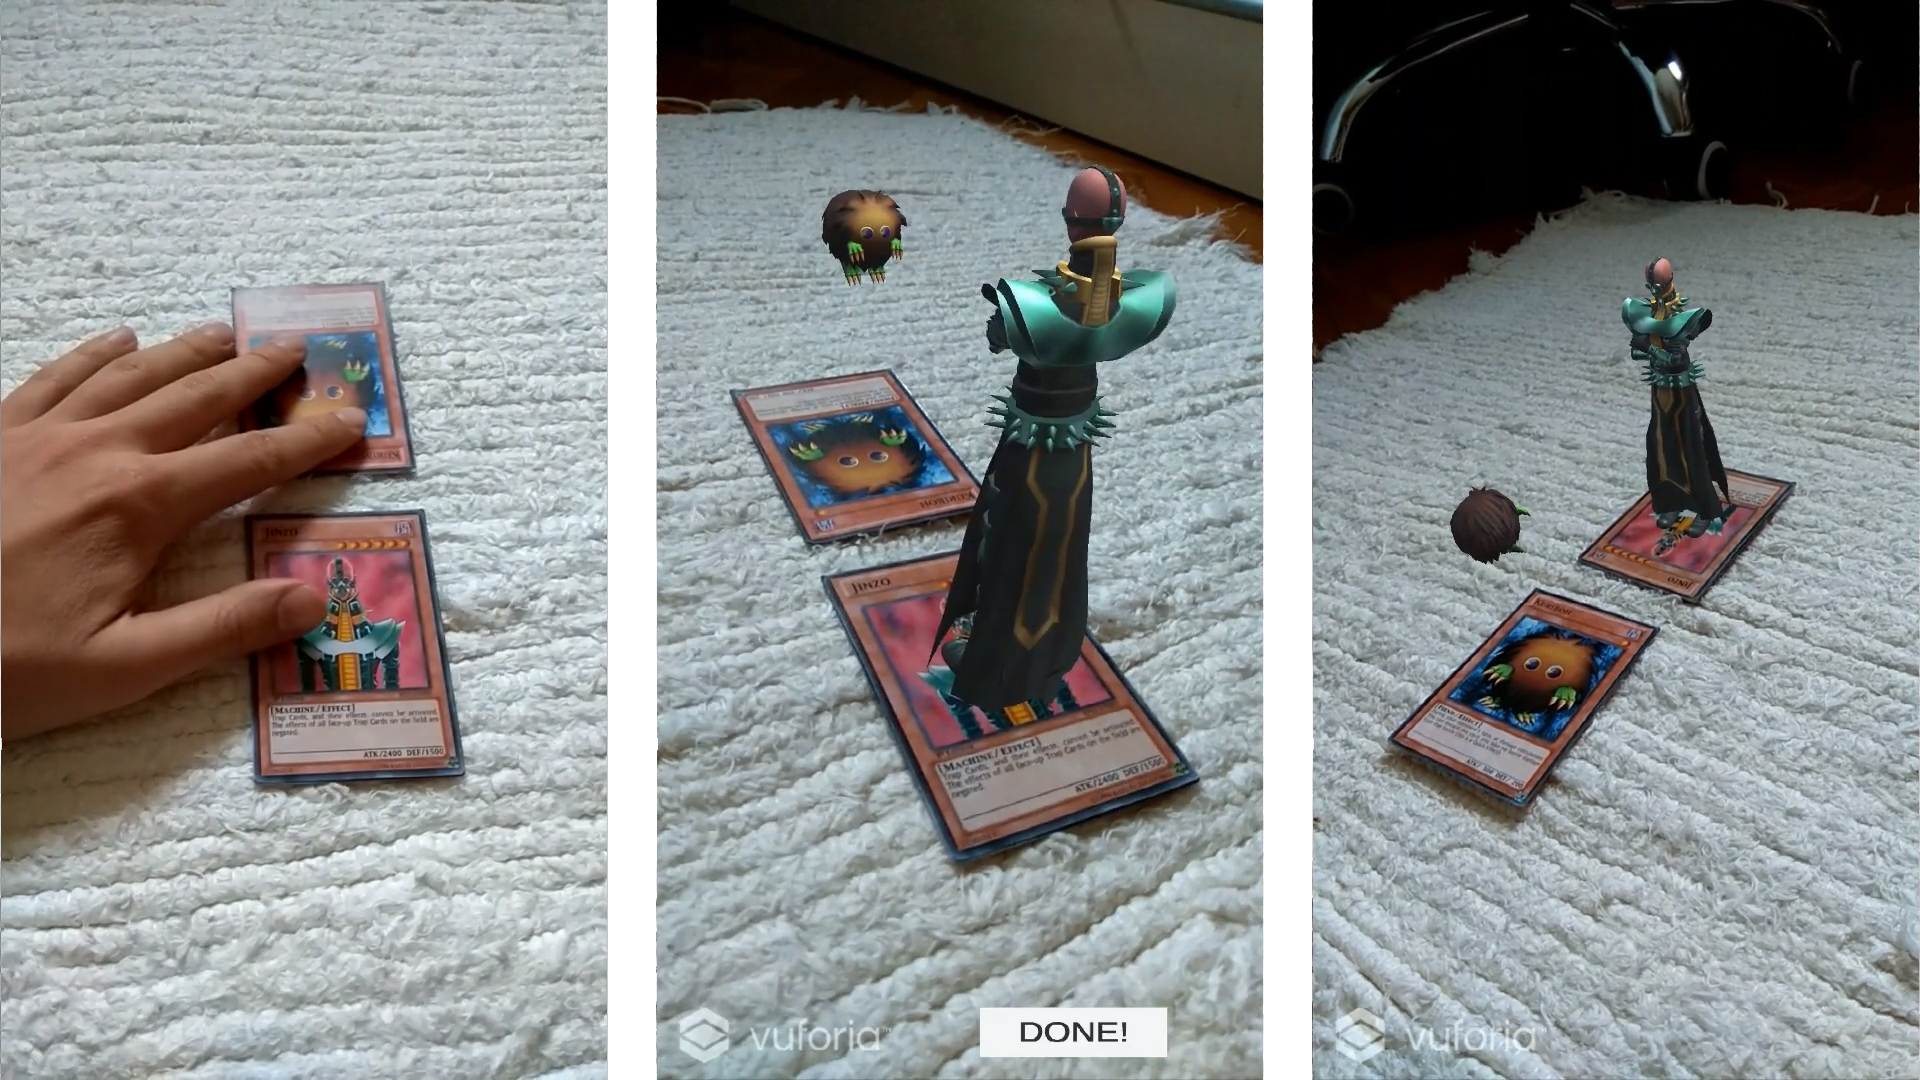
\includegraphics[width=\linewidth]{Images/YuGiOh.jpg}
    \caption{Visualización del juego de cartas}
    \label{YuGi}
\end{figure}

\textbf{Se pueden ver los resultados en el video \url{https://vimeo.com/331237916}.}\\

Con estas pequeñas muestras habríamos terminado nuestra incursión en la realidad aumentada con marcadores y estaríamos preparados para el siguiente paso, en el que prescindiríamos de ellos.

\newpage
\subsection{JengAR}
Una de las opciones para el juego multijugador online fue implementar el famoso juego de mesa Jenga\cite{jenga} en realidad aumentada con \textit{cloud anchors}. \\
Decidimos desarrollar un prototipo rápido donde se instancia una pila de bloques en un plano. Si nos acercamos un bloque y mantenemos pulsado la pantalla, el bloque se ancla a nuestro movimiento, por lo que hay que realizar movimientos suaves y cuidadosos, para no tirar la torre.\\
Cuando se pulsa la pantalla se calcula el punto que se encuentra en la mitad de la pantalla y se lanza un \textit{raycast} \footnote{Rayo que se lanza desde un punto origen hasta un punto final para comprobar si existe algún elemento en el camino}, si éste detecta un bloque, se marca como seleccionado, se fija la distancia entre su posición y la nuestra, y empieza a moverse junto a nosotros, manteniendo la distancia inicial.\\
En la figura \ref{JenAR} se pueden observar algunas capturas de la aplicación.
\begin{figure}[H]
    \centering
    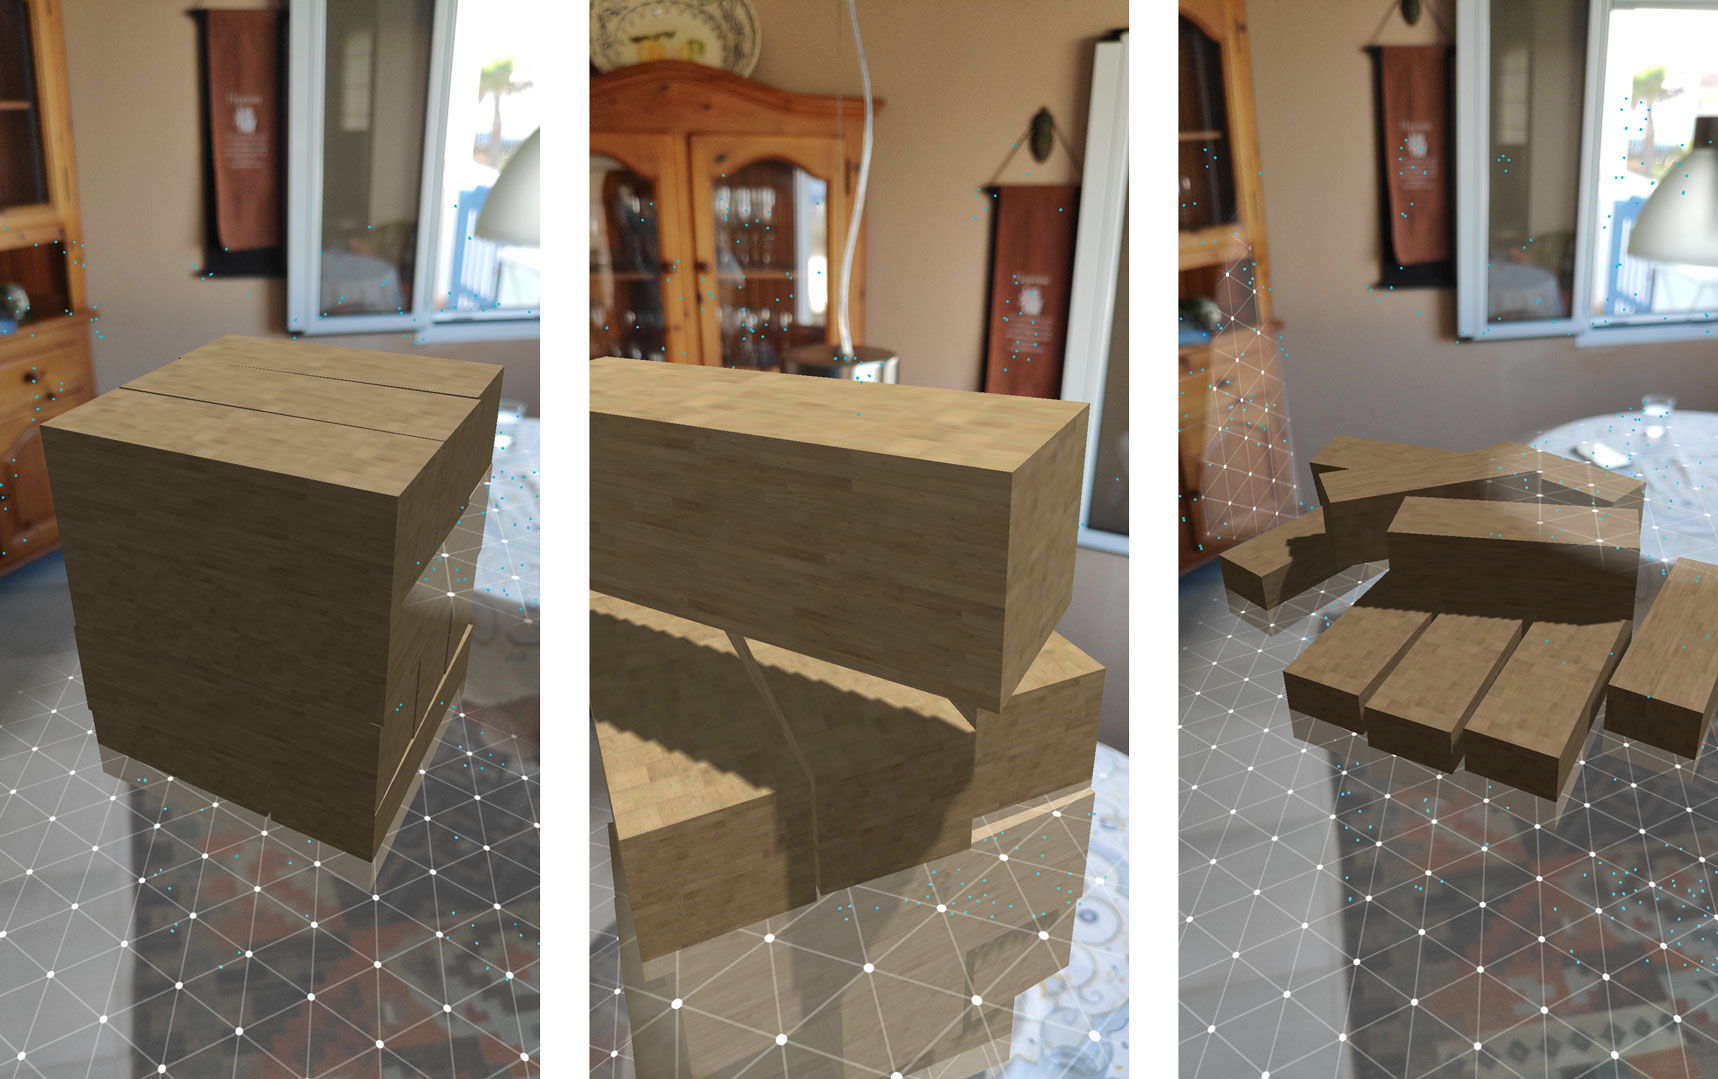
\includegraphics[width=\linewidth]{Images/Jenga.jpg}
    \caption{Visualización del JengAR}
    \label{JenAR}
\end{figure}
Optamos por abandonar el desarrollo debido a su poca complejidad, ya que la implementación era demasiado sencilla, por lo que no llegamos a implementar la mecánica de turnos ni la detección de victoria o derrota.\\

\newpage
\section{Juego multijugador con \textit{cloud anchor} - BombARdero+}
La tecnología que mas nos ha impresionado ha sido los \textit{Cloud Anchors}, nunca habíamos oído hablar de ella. Cuando nos enteramos de su existencia, estábamos todos de acuerdo en desarrollar un videojuego multijugador \textit{online}.\\

Los Cloud Anchors, como hemos explicado anteriormente, se almacenan en la nube de Google. Para usarlos, hace falta conseguir una clave de licencia de \textit{ARCore Cloud Anchor API} en Google Cloud Platform \cite{GCloud}. Una vez conseguida la credencial, hay que introducirla en Unity3D, ``Edit -> Project Settings -> Google ARCore -> Cloud Anchor API Keys''. En los ejemplos que ofrece Google, la implementación de los Cloud Anchor utiliza la \textit{Multiplayer High Level API(Multiplayer HLAPI)} de Unity, por lo que también hay que activar el servicio de multijugador en nuestro proyecto desde el \textit{dashboard} de Unity \cite{UnityDashboard}. Una vez realizado estos dos pasos, al compilar la escena de ejemplo, debería funcionar. En esa escena, un usuario tiene que crear una sala e instanciar un objeto, el punto de anclaje principal, que se convertirá en las coordenadas (0,0,0) del entorno.
Este punto de anclaje tarda unos diez segundos en subirse a la nube y estar disponible para más usuarios, que al entrar a la aplicación le aparece un listado con las salas disponibles. \\

Para desarrollar este juego, primero desarrollamos dos aplicaciones anteriormente.

Como al principio no teníamos dos móviles que soportasen ARCore, programamos el juego en monojugador, para acostumbrarnos al entorno y para ahorrarnos trabajo en un futuro.\\

En paralelo, como teníamos que implementar la parte de multijugador online y no teníamos ningún tipo de experiencia, realizamos unas pruebas para estudiar el funcionamiento de la Multiplayer HLAPI. Esas pruebas nos permitieron entender y aprender a desarrollar el multijugador de la prueba de concepto que nos hemos puesto como objetivo.\\

Una vez que conseguimos tener dos dispositivos que soportasen ARCore, empezamos a desarrollador la aplicación multijugador. Gracias a haber desarrollado el \textit{BombARdero}, nos permitió avanzar muy rápido ya que estaban los modelos, \textit{prefabs}\footnote{ Objetos prefabricados de Unity3D}, y scripts con las mecánicas básicas ya creadas. Primero tuvimos que mirar como estaba montada la implementación de Google, para entender el proceso de cómo se subía el marcador a la nube y la cantidad de información de control que teníamos. Este proceso fue bastante sencillo, ya que el código de ejemplo es muy entendible e intuitivo. Una vez conseguido implementar el BombARdero con los Cloud Anchors, hubo que hacer unos pequeños retoques a los scripts y añadir componentes de la multiplayer HLAPI a los objetos, para implementar la parte multijugador.\\

En el \textit{Cloud Anchor Network Manager} hay que registrar el objeto que se va a instanciar cada vez que entra un jugador a la partida, en nuestro caso será un avión. El avión en un principio está desactivado y se activa en el momento en el que se \textit{hostea} o resuelva el anchor principal. El avión consta de una velocidad constante hacia delante, y para controlar su trayectoria existe en la parte inferior izquierda de la pantalla un \textit{joystick} que te permite mover el avión hacia arriba, abajo, derecha e izquierda. En la esquina inferior derecha se encuentra un botón que al pulsarlo, se lanza una bomba en la posición del avión, dicha bomba sirve para destruir los edificios que se encuentran en la ciudad. El objetivo principal del juego es destruir el mayor número de edificios posible.

La principal complicación fue implementar la parte de multijugador, ya que no teníamos conocimiento previo sobre el tema.


\clearpage
\section{Instrucciones de montaje de muebles en AR - AmueblAR}

En nuestra investigación hemos visto que una de las utilidades más populares actualmente en el campo de la realidad aumentada son las aplicaciones de decoración de interiores. Ikea, por ejemplo, ha lanzado Ikea Place, una aplicación de realidad aumentada para dispositivos móviles que permite visualizar cualquier habitación de tu casa con muebles virtuales. De esta manera podemos decidir si encajan con nuestro salón y si las medidas son las adecuadas para después comprar el mueble en la tienda física.\\

Este programa despertó nuestra curiosidad y pensamos que podríamos desarrollar una aplicación con una utilidad parecida, pero en este caso aplicada al montaje de los muebles. Sabemos que comprar sofás o estanterías por piezas es en ocasiones más barato y facilita enormemente el transporte, sin embargo la parte en la que muchos compradores experimentan problemas es a la hora de montarlos. Muchos son incapaces de ver en el plano de las instrucciones en qué lugar va cada tornillo o de qué forma se unen las patas. Por eso, la aplicación que nosotros hemos propuesto consiste en un pequeño manual de instrucciones en realidad aumentada sin marcadores. De esta manera se puede ver en todo momento el modelo 3D del mueble, rotarlo y además desplazarte alrededor de él para apreciar en detalle cada uno de los pasos en el proceso de montaje.\\

El funcionamiento es muy sencillo: para empezar escaneamos el plano para que el programa cree una superficie donde colocar el mueble. A continuación tocamos la pantalla en el lugar en el que queremos colocarlo. Ahora podemos rotar el mueble hacia izquierda y derecha para dejarlo en una posición en la que nos resulte cómodo acercarnos y alejarnos mientras vemos los pasos de montaje. Finalmente, al pulsar el botón de aceptar entramos en la fase de construcción. En ella tenemos un botón a cada lado de la pantalla: el de la izquierda retrocede al paso anterior y el de la derecha avanza al paso siguiente. Mientras se suceden las animaciones que van explicando cómo armar progresivamente el mueble el usuario puede moverse libremente con su dispositivo para apreciar los detalles e incluso retroceder si no ha entendido bien el paso a seguir.\\

Para el desarrollo hemos utilizado la librería ARCore, que permite el despliegue de realidad aumentada sin marcadores. Utilizando la tecnología que nos vienen dada por la librería buscamos una serie de puntos en el suelo que nos permitirán crear un plano virtual. Una vez generada esta superficie el plano se representa gráficamente en pantalla con la unión de los puntos. A continuación dividimos la aplicación en tres estados: despliegue, rotación y montaje.\\ 

Empezamos en la fase de despliegue, en la que el programa está continuamente esperando la interacción del usuario. Cuando se toca la pantalla, se comprueba si ha habido colisión con el plano virtual, y de ser así se instancia el mueble en el lugar en el que hemos tocado. Si este proceso se ha llevado a cabo con éxito, pasamos a la fase de rotación. Aquí aparecen dos botones azules a los lados de la pantalla y uno verde en la parte inferior. Los botones laterales llevan una referencia al mueble para que al ser pulsados lo roten en una u otra dirección. El botón inferior por otra parte nos sirve para comunicarle a la aplicación que estamos conformes con la posición actual del objeto y que puede pasar a la siguiente fase.\\ 

Finalmente nos encontramos con dos nuevos botones a los laterales, que como hemos explicado anteriormente se encargan de adelantar y retroceder los pasos de montaje. El sofá tiene un componente \textit{Animator Controller} que lleva el árbol de estados. Este árbol consta de 10 estados fijos, en los que se queda el mueble una vez ha terminado su animación correspondiente y 18 estados móviles o animaciones, que se reproducen cuando pulsas el botón de avanzar o retroceder. Para ello, existe una variable que controla el avance y otra que hace lo propio con el retroceso, que se anulan una vez se entra en un estado estático y se activan al pulsar el botón que corresponde, pasando así a la animación del paso siguiente o anterior.\\

Cabe destacar el proceso de creación del mueble en sí mismo, que en el caso del ejemplo se trata del sofá \textit{Kivik}. Como no era posible encontrar un modelo dividido en piezas y fácilmente animable tuvimos que modelarlo desde cero con la ayuda de la documentación que encontramos en la web de Ikea. El mueble consta de las siguientes piezas: el asiento del sofá, el respaldo del sofá, el asiento de la \textit{cheslong} \footnote{ Tipo de sofá que posee una prolongación lo suficientemente larga en forma de L como para soportar las piernas humanas.} y su respaldo, los dos brazos, dos escuadras, una pletina, ocho patas, dieciocho tornillos con sus correspondientes tuercas y arandelas, cinco cojines cuadrados y un cojín alargado para la \textit{cheslong}. Excluyendo los tornillos, que los encontramos en una página de recursos gratuitos \cite{tornillos}, todos los demás fueron creados por nosotros en Blender, herramienta de la que ya hemos hablado anteriormente. Una vez terminadas las piezas del sofá, las texturizamos con colores azules y aspecto de sofá, y por otro lado las piezas como los tornillos o las escuadras una textura metálica.\\

Pensamos que podríamos empezar a animar cada parte por separado dentro de un objeto conjunto del que fueran hijas todas las piezas, pero para que Unity pueda interpretar cada acción como propia de un objeto mayor a las partes es necesario hacer un \textit{rigging}\footnote{ Proceso de crear un sistema de controles digitales y agregárselos a un modelo 3D para que así pueda ser animado fácilmente y eficientemente} que abarque todas piezas del sofá. Una vez construido el esqueleto hay que asignarle a cada hueso el objeto que se va a encargar de mover, lo cual dio también algunos problemas, ya que al tratarse de un objeto conjunto ciertos huesos acababan emparentándose automáticamente con partes del sofá que nos les correspondían, de modo que la única solución fue establecer manualmente los pesos (es decir, la influencia que tiene cada hueso sobre una parte concreta) sobre los diferentes conjuntos de vértices hasta que conseguimos el resultado que esperábamos.\\

En lo referente a las animaciones nos fue muy útil el vídeo que tiene publicado la cuenta de Ikea España en la plataforma Youtube \cite{IkeaYT} en el que se explica el procedimiento que se sigue para construir el sofá. Habiéndolo analizado dividimos el montaje en 9 pasos diferenciados y los animamos también en Blender, haciendo desaparecer las partes que no se están utilizando en ese momento para que sea más claro y fácil verlo.\\

Al contrario que en los ejemplos con marcadores en los que pudimos exportar directamente el archivo de Blender para su uso en Unity, aquí nos dio problemas ya que el editor dejó de reconocer los \textit{clips} de vídeo de algunas animaciones. Solventamos este problema exportando el objeto desde el programa de modelado en formato ``fbx'', pero nos surgió otro nuevo inconveniente, todas las partes del sofá habían perdido sus texturas. Ya desde Unity creamos los materiales por separado y se los asignamos a cada pieza.
Fue un proceso bastante agotador, sobre todo en la parte artística, pero consideramos que el resultado es satisfactorio y útil, además ofrece nuevas posibilidades en un campo que no deja de crecer.

\clearpage
\section{Visualizador de objetos en AR con gafas Aryzon}
En la fase de investigación, pensamos que una de las limitaciones de la realidad aumentada en dispositivos móviles es el hecho de tener que que estar sujetando el móvil con las manos, por lo que el control y la experiencia de usuario se ve condicionada negativamente. Decidimos buscar un headset de realidad aumentada encontramos las gafas de Aryzon \cite{Aryzon}, compramos un ejemplar y probamos qué tal funcionaban.\\

Descargamos las aplicaciones y juegos que promocionan para ver como era la experiencia usando las gafas. Nos resultó curioso y decidimos desarrollar una aplicación en la que se pudiera ver objetos y/o modelos 3D y poder caminar alrededor de ellas. Para añadirle más funcionalidad, usamos un mando de \textit{Xbox One} que nos permitirá mover, rotar y escalar el modelo a nuestro gusto, con el objetivo de poder manipular la aplicación sin necesidad de tocar el móvil, ya que éste estará colocado en las gafas.\\

Para el desarrollo de la aplicación usamos el SDK de Aryzon, que nos facilita la vista estereoscópica\footnote{ Dos puntos de vista poco separados entre sí} para simular nuestros ojos, ya que las gafas están compuestas por dos espejos que reflejan la imagen al cristal por donde nosotros vemos el mundo real, permitiendo tener esa visión de realidad aumentada como se puede observar en la figura \ref{GafasAryzon}.

\begin{figure}[H]
    \centering
    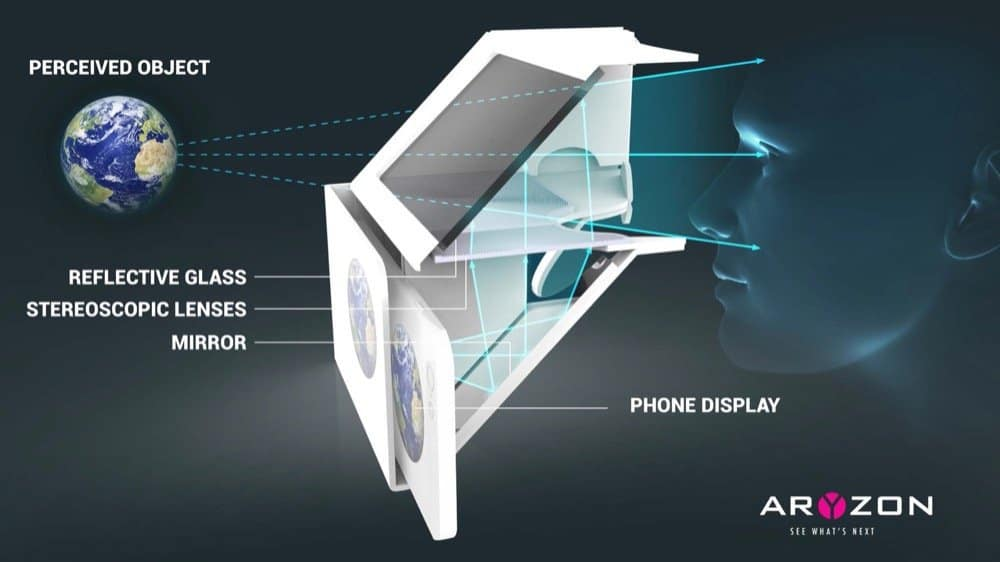
\includegraphics[width=0.75\linewidth]{Images/How-it-works.jpg}
    \caption{Como funciona las gafas de Aryzon}
    \label{GafasAryzon}
\end{figure}
 {\let\thefootnote\relax\footnote{{Imagen de la figura \ref{GafasAryzon} sacada de https://www.igadgetsworld.com/aryzon-diy-augmented-reality-headset/}}}

Todos los ejemplos que proporciona Aryzon son con marcadores o no usan de verdad realidad aumentada, si no que que es una escena de realidad virtual con fondo negro y vista esteoroscópica, entonces da el efecto de ser realidad aumentada, pero la aplicación en sí es realidad virtual. Nosotros hemos decidido usar ARCore, ya que queremos usar la realidad aumentada sin marcadores y movernos alrededor del modelo, y como hemos visto en las pruebas, la estabilidad de los puntos de anclaje de ARCore es muy buena.\\
Para el desarrollo de esta prueba de concepto, necesitamos el SDK de Aryzon y el SDK de ARCore, y los modelos sacados del \textit{Asset Store} de Unity \cite{AssetStore}. Desarrollamos un \textit{script} para manipular con el mando de Xbox One los objetos que instanciamos. El joystick izquierdo sirve para mover el objeto en los ejes X y Z, para moverlo verticalmente, se usa la cruceta (D-PAD) vertical. Para rotar el objeto en cuestión hemos configurado el script para que se realice con el joystick derecho, y para finalizar, con la cruceta horizontal podemos escalar el objeto. Por otro lado, los botones con los que controlamos la creación de objetos son, la A que permite instanciar el objeto en el lugar en el que estemos mirando, la X que cambia el modelo que se va a instanciar, ya que hemos puesto seis modelos en esta prueba de concepto y la B, nos permite activar y desactivar el \textit{render} de los planos que ha encontrado la aplicación, para tener una visión más limpia.\\
El mayor problema que nos encontramos al desarrollar la aplicación fue la documentación respecto al \textit{mapeo} del mando, ya que cambia según la plataforma en la que se utiliza. La de Android no estaba actualizada y no coincidían los botones y los ejes que nos proporcionaba la documentación.\\
El resultado final nos parece muy interesante, ya que tener el teléfono fijo en nuestros ojos gracias a las gafas, hace que podamos tener las manos libres para poder controlar y manipular lo que queramos ver. El precio de las gafas es un precio asequible para el público, y en nuestro caso hemos utilizado un mando de \textit{Xbox One} oficial, pero existen mandos Bluetooth para los \textit{smartphones} que también se pueden conseguir muy baratos. Usando la realidad aumentada de esta manera abre las posibilidades a nuevas mecánicas de juego y seguramente suponga una revolución en la realidad aumentada de "bolsillo".\\
Lo que se ve en la figura \ref{appAryzon} es la aplicación usando ARCore y el SDK de Aryzon, el modelo que vemos en la imagen, se proyecta a traves del sistema de cristales explicado anteriormente, permitiendo una visión del mundo real y el modelo 3D superpuesto en el plano encontrado.

\begin{figure}[H]
    \centering
    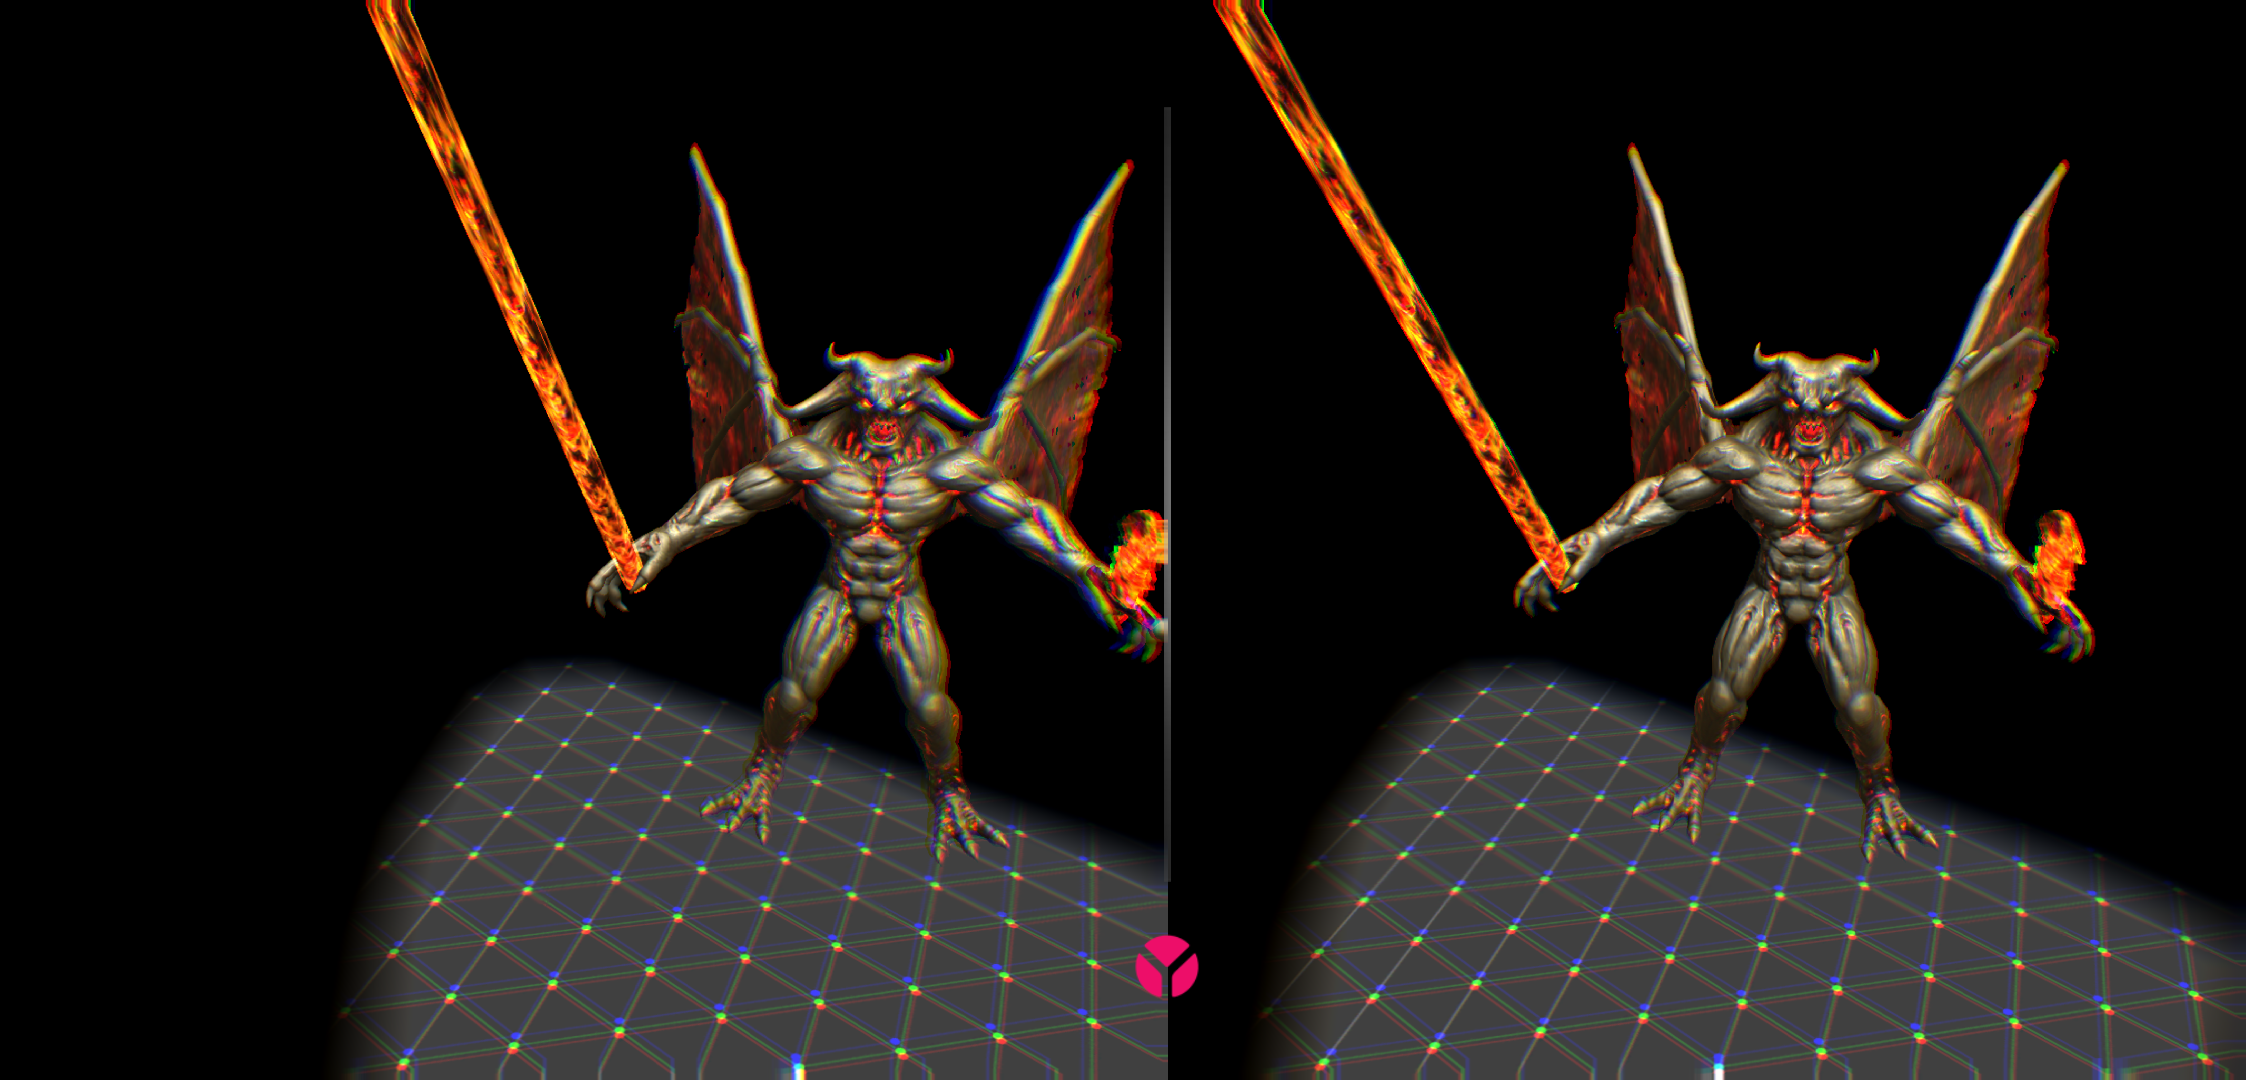
\includegraphics[width=0.75\linewidth]{Images/aryzonVisualizer.png}
    \caption{Proyección estereoscópica del móvil}
    \label{appAryzon}
\end{figure}
\noindent